\section{RP14 Unobtrusive JavaScript}
\label{sec:principle-rp14-unobtrusive-javascript}

Aktuelle Webapplikationen können grob in zwei Kategorien eingeteilt werden:

\begin{figure}[H]
	\begin{table}[H]
		\tablestyle
		\tablealtcolored
		\begin{tabularx}{\textwidth}{l l X}
			\tableheadcolor
				\tablehead Kategorie &
				\tablehead Beispiel &
				\tablehead Erläuterung
				\tabularnewline
			\tablebody
				Statisch &
				\emph{GitHub} \cite{GitHub} &
				User Interface wird auf dem Server gerendert, JavaScript bringt lediglich dynamisch geladene Inhalte, Effekte oder zusätzliche ``optionale'' Features.
				\tabularnewline

				JavaScript Client &
				\emph{Google Drive} \cite{GoogleDrive} &
				User Interface wird komplett im Browser mittels JavaScript aufgebaut. Ohne JavaScript keine Funktionalität oder schlechtere User Experience.
				\tabularnewline
			\tableend
		\end{tabularx}
	\end{table}
	\caption{Kategorisierung aktueller Webapplikationen}
	\label{tab:current-webapplication-categories}
\end{figure}

Die Kategorie \emph{Statisch} zeichnet sich durch hohe Kompatibilität mit allen möglichen Internetbrowsern aus. Durch die Generierung des HTML Markups losgelöst vom schlussendlichen Zielclient, liegt die ganze Verantwortung, vom Beschaffen anzuzeigender Daten bis hin zum Zusammenstellen des HTML \gls{DOM}'s komplett bei der Serverkomponente.

Zwar kommt auch bei diesem Typus oftmals JavaScript zur Anwendung, meist beschränkt sich dessen Anwendung aber auf die Ergänzung des bereits statisch geladenen Inhaltes. So lädt \emph{Mila} \cite{Mila} beim Seitenwechsel, sofern JavaScript aktiviert ist, neue Inhalte über einen \gls{AJAX} Request. Nach Erhalt des vorgerenderten HTML Markups aus der Antwort ersetzt JavaScript entsprechende Inhalte im aktuell angezeigten HTML \gls{DOM} des Browsers.

Als Programmiersprache auf dem Applikationsserver kommt hier oft Java, Python, PHP, Ruby o.Ä. zum Einsatz.

Beim puren \emph{JavaScript Client} liegt der Programmcode für das Rendern des User Interfaces mit all seinen Inhalten als JavaScript Quelltext vor. Nach erfolgreicher Übertragung zum Internetbrowser initiiert dieser die Erstellung der Applikationsoberfläche im HTML \gls{DOM} des Clients.

Sollen dynamische Informationen angezeigt werden, müssen diese über eine Serviceschnittstelle beim entsprechenden Anbieter angefragt werden (siehe bspw. Abschnitt \ref{sec:principle-rp1-rest} ``\nameref{sec:principle-rp1-rest}'').

Die Verlagerung des User Interface Quelltexts direkt in den Browser hat den Vorteil, dass UI Elemente effizienter verändert und aktualisiert werden können. Soll bspw. nur ein kleiner Teil der Benutzeroberfläche aktualisiert werden, kann dies gezielt und ohne Umweg über einen erneuten Request an den Server geschehen.

Durch diese Vereinfachung entfallen unnötige Wartezeiten zwischen Benutzereingabe und Systemreaktion. Dies resultiert wiederum in einer verbesserten User Experience.

Es ist bereits zu erahnen, dass diese Art von Webapplikation ohne JavaScript-Unterstützung im Browser nicht ausgeführt werden kann. Ein Beispiel hierfür liefert der \emph{Google Drive} \cite{GoogleDrive} Webclient. Wie in Abbildung \ref{fig:googleDriveNoJs} ersichtlich verweigert dieser ohne aktiviertes JavaScript die Funktion und zeigt ein leeres Standardlayout mit einer entsprechenden Meldung an.

\begin{figure}[H]
	\centering
	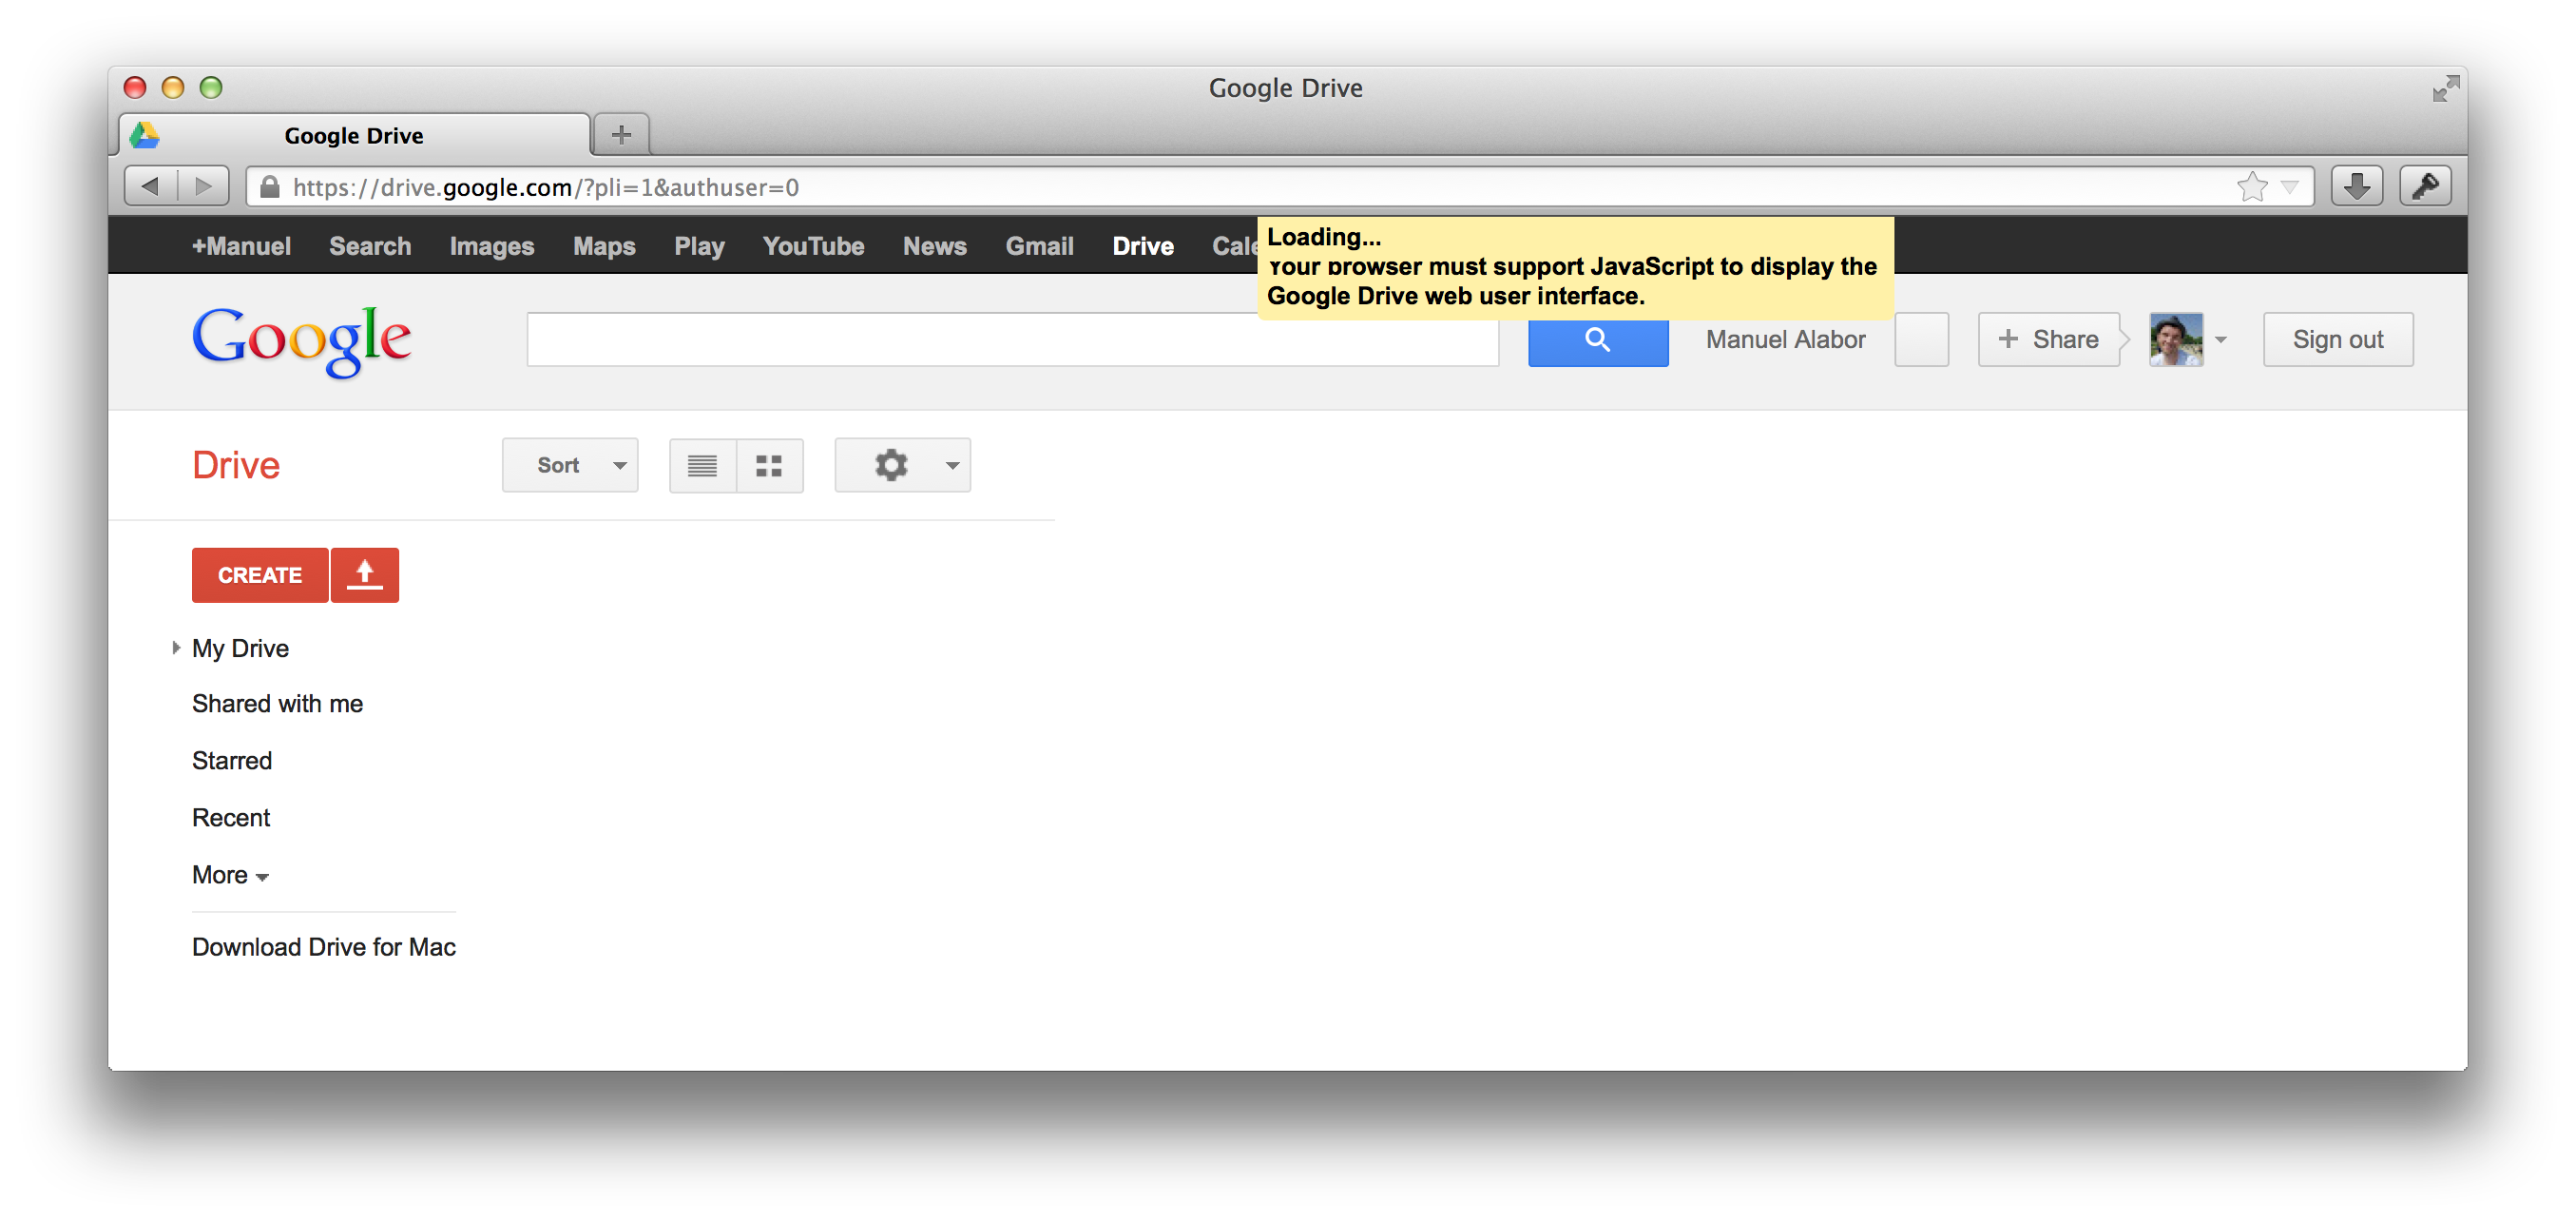
\includegraphics[width=12cm]{content/principle-demonstration/images/googledrive-nojs.png}
	\caption{\emph{Google Drive} in Firefox 21.0 mit deaktiviertem JavaScript}
	\label{fig:googleDriveNoJs}
\end{figure}

Die Richtlinie \emph{RP14 Unobtrusive JavaScript} aus dem ROCA Manifest verlangt, dass eine Webapplikation auch bei deaktiviertem JavaScript weiter funktionstüchtig bleibt. Soll JavaScript für ein modernes User Interface verwendet werden, muss gem. \emph{RP14} also eine Mischform aus den vorgestellten Applikationstypen verwendet werden.
\newline\newline
Neben dem ``Wie und Wo'' ein User Interface gerendert wird, ist die Richtlinie \emph{Unobtrusive Javascript} auch eng mit der Thematik \emph{Codequalität} verbunden: Die Vermengung von HTML Markup und JavaScript Code soll unterbunden werden. Hierzu zeigt der Quelltext \ref{lst:badHtmlMarkupWithJavaScript} ein Beispiel, wie es unter keinen Umständen umgesetzt werden sollte.

\begin{lstlisting}[language=HTML, caption={Beispiel einer Vermischung von HTML Markup und JavaScript}, label={lst:badHtmlMarkupWithJavaScript}]
<a href="adresses.html" onClick="$('#progressIndicator').removeClass('hidden');showAddresses();return false;">
	Display Addresses
</a>
\end{lstlisting}

In den Quelltexten \ref{lst:goodHtmlMarkupWithoutJS} und \ref{lst:goodJSOutsideHtmlMarkup} ist ersichtlich, wie eine Separierung von JavaScript Logik und HTML Markup optimal implementiert wird.

\begin{lstlisting}[language=HTML, caption={Beispiel eines sauberen HTML Markups ohne JavaScript}, label={lst:goodHtmlMarkupWithoutJS}]
<a href="adresses.html" id="showAddresses">Display Addresses</a>
\end{lstlisting}

\begin{lstlisting}[language=JavaScript, caption={Beispiel Event-Handler in ausgelagerter JavaScript Datei}, label={lst:goodJSOutsideHtmlMarkup}]
$(function() {
	$('#showAddresses').on('click', showAddresses);

	function showAddresses() {
		$('#progressIndicator').removeClass('hidden');
		// ... show addresses
		return false;
	}
});
\end{lstlisting}


\subsection*{Geplante Umsetzung}

Als Herausforderung hat das Projektteam geplant, die Beispielapplikation \emph{Roomies} als Mischung der vorgestellten Applikationstypen umzusetzen.

Grundsätzlich sollen Inhalte statisch auf der Backendkomponente gerendert werden. Hat der Benutzer in seinem Browser JavaScript aktiviert, ermöglicht der entsprechender Programmcode die Umsetzung der im einleitenden Abschnitt vorgestellten Funktionalitäten eines vollwertigen \emph{JavaScript Clients}.

Zugriffe auf persistente Applikationsdaten sollen wie in \ref{sec:principle-rp1-rest} ``\nameref{sec:principle-rp1-rest}'' vorgeschlagen in ein entkoppeltes Serviceinterface gekapselt werden.

Um die Wartbarkeit der Codebasis zu optimieren, soll die Separierung von HTML Markup und JavaScript wie beschrieben strikt eingehalten werden.


\subsection*{Konkrete Umsetzung}

Während der Implementation der geplanten Lösung wurde sehr schnell klar, dass die entstehende Applikation zwar wie erwartet die gewünschte hybride Form aufweisen wird, aber keinesfalls mit der ROCA Richtlinie \emph{\nameref{sec:principle-rp15-no-duplication}} vereinbar sein wird.

Dank der durchgängigen Verwendung von JavaScript hätten viele Codefragmente wie die View-Templates (Beispiel siehe Quelltext \ref{lst:reusableHandlebarsViewTemplate}) auch im Frontend wiederverwendet werden können. Andere, logikintensivere Komponenten wie die Controller zur Steuerung der eigentlichen User Interface Funktionalitäten (Event-Handling, Datenzugriffe etc.) hätten doppelt implementiert werden müssen.

\newpage
\begin{lstlisting}[language=JavaScript, firstnumber=31, caption={Ausschnitt aus dem \emph{Handlebars} \cite{Handlebars} Template zur Darstellung von Benutzerinformation in der Menüleiste von \emph{Roomies} \cite{roomiesMenuTemplate}}, label={lst:reusableHandlebarsViewTemplate}]
{{#if user}}
<ul class="right">
	<li class="account">
		<a href="/resident/{{user.facebookId}}/profile">
			<span class="item-label">{{user.name}}</span>
			<img class="avatar small" src="//graph.facebook.com/{{user.facebookId}}/picture" />
		</a>
	</li>
</ul>
{{/if}}
\end{lstlisting}

Um diesem Umstand gegensteuern zu können teilte sich das Projektteam nach der ersten Entwicklungsiteration in zwei Gruppen:

\begin{itemize}
	\item Zwei Mitglieder arbeiteten weiter an der Umsetzung der geplanten Use Cases
	\item Ein Mitglied fokussierte sich auf die Entwicklung einer Möglichkeit, identischen Applikationscode sowohl in der Backend-Komponente für statisches Rendering als auch direkt im Browser als JavaScript Client verwenden zu können.
\end{itemize}

Aus diesem Prozess entstand das eigenständige Framework \emph{barefoot} \cite{Barefoot}. Es setzt auf der verbreiteten Bibliothek \emph{Backbone.js} \cite{Backbonejs} auf und ermöglicht die Verwendung einer einzigen, einheitlichen Codebasis für JavaScript-basierte Webapplikationen (siehe dazu auch Kapitel ``\nameref{sec:sad}'' Abschnitt \ref{sec:sad-implementation}).

Mit der Integration des neuartigen Frameworks kann komplett auf doppelte Codefragmente verzichtet werden. Gleichzeitig profitiert der Endbenutzer von kurzen Lade- und Reaktionszeiten im User Interface. Sollte auf dem Client kein JavaScript verfügbar sein, greift automatisch das klassische servergestützte Rendering und alle Funktionalitäten bleiben zugänglich.

Zwar gibt es mit \emph{Rendr} von \emph{Airbnb} \cite{Rendr} eine Konkurrenzbibliothek auf diesem Gebiet. Aufgrund einiger, insbesondere designbedingter Nachteile, entschied das Projektteam jedoch, mit \emph{barefoot} eine eigene Implementation umzusetzen:

\begin{figure}[H]
	\begin{table}[H]
		\tablestyle
		\tablealtcolored
		\begin{tabularx}{\textwidth}{X X}
			\tableheadcolor
				\tablehead Problem von Rendr &
				\tablehead Lösung durch barefoot
				\tabularnewline
			\tablebody
				Unterstützt nur \emph{Handlebars} \cite{Handlebars} für View-Templates &
				Keine Vorgabe resp. ohne Template-Engine verwendbar
				\tabularnewline

				Quelltext für Client kann nicht automatisch zusammengefasst und zur Übertragung optimiert werden &
				\emph{Barefoot} verwendet hierfür die \emph{browserify-middleware} (siehe auch \ref{sec:principle-rp17-static-assets} ``\nameref{sec:principle-rp17-static-assets}'')
				\tabularnewline

				\emph{Rendr} ist mittels \emph{CoffeeScript} \cite{CoffeeScript} implementiert &
				\emph{Barefoot} setzt auf pures JavaScript unter Verwendung von \emph{Underscore} \cite{Underscore}
				\tabularnewline

				Wiederholte Überprüfung der aktuellen Runtime-Umgebung (Client oder Server) mittels entsprechender \emph{if}-Statements &
				Einmalige Überprüfung, anschliessende Verwendung umgebungsspezifischer \gls{Mixin}s
				\tabularnewline
			\tableend
		\end{tabularx}
	\end{table}
	\caption{\emph{Rendr} vs. \emph{barefoot}}
	\label{tab:rendr-vs-barefoot}
\end{figure}


\subsection*{Diskussion}

Ähnlich den zwei Typen von Webapplikationen sind hier zwei kontroverse Strömungen in der Entwicklergemeinschaft erkennbar \cite{StackOverflowUnobtrusiveJavascriptOutdated}: Die eine Gruppe drängt zur alleinigen Nutzung der neusten Features und tendiert daher eher zu Lösungen mit reinen \emph{JavaScript Clients}. Andere Gruppierungen geben sich vergleichsweise konservativ. Sie argumentieren damit, dass:

\begin{itemize}
	\item zum Einen die Kompatibilität zu weniger leistungsstarken Browsern resp. JavaScript Engines (Smartphones, alte Browserversionen etc.) gewährleistet sein müsse
	\item zum anderen die Umsetzung einer ebensolchen \emph{unobtrusive} Lösung entsprechend aufwändig sei.
\end{itemize}

Beiden Lagern kann das Projektteam mit der umgesetzten Beispielapplikation entgegentreten: Mit \emph{barefoot} sind Webapplikationen möglich, welche mit einer einzigen, durchgängigen Codebasis sowohl das statische als auch clientseitige Rendering von User Interfaces resp. deren Ausführung ermöglicht. Daraus resultiert eine im Vergleich zur doppelten Implementierung höhere Effektivität im Entwicklungsprozess. Gleichzeitig kann das Erlebnis für den Endbenutzer optimiert werden.

Ob sich die Investition in die Entwicklung einer Webapplikation, welche \emph{RP14 Unobtrusive JavaScript} genügt, lohnt, kann das Projektteam nicht pauschal beantworten. Je nach Anforderungen kann die Erfüllung dieser Richtlinie aber zu einer höheren Akzeptanz bei den Benutzern führen. Frameworks wie \emph{barefoot} können zudem künftig dazu beitragen, einfacher eine ``unobtrusive'' Lösung umzusetzen.
